\begin{figure}
	\centering
	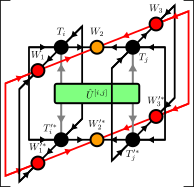
\includegraphics[scale=1]{figures/tikz/YB_isoTPS/tebd_environment/tebd_environment.pdf}
	\caption{The cost function of the optimization problem \eqref{eq:YB_isoTPS_TEBD_maximizing_overlap} that must be solved for locally applying TEBD operators $\hat{U}^{[i,j]} \coloneqq \hat{U}^{[i,j]}(\Delta t)$ can be computed as a contraction of the two-site wave functions of $\ket{\Psi}$ and $\ket{\Psi^\prime}$, sandwiching the operator between the two.}
	\label{fig:YB_isoTPS_TEBD_overlap_contraction}
\end{figure}
Let us assume that the orthogonality center is positioned between the two sites on which the bond operator $\hat{U}^{[x, y]}\left(\Delta t\right)$ acts. The five tensors around the orthogonality center then make up a sub-network with only incoming arrows, compare Figure \figref{fig:YB_isoTPS_twosite_expectation_value_environment}. We call these five tensors $T_1$, $T_2$, $W_1$, $W_2$ and $W_3$. The local TEBD update can then be formulated as the following problem: Find tensors $T_1^\prime$, $T_2^\prime$, $W_1^\prime$, $W_2^\prime$ and $W_3^\prime$ satisfying the isometry constraints and minimizing the error
\begin{equation}
	\label{eq:isoDTPS_TEBD_local_update_error}
	\varepsilon_\text{trunc} = \left\lVert \hat{U}^{[x,y]}(\Delta t)\ket{\Psi} - \ket{\Psi}\right\rVert
\end{equation}
Similar to the YB-move, we can rewrite this as the problem of maximizing the overlap
\begin{equation}
	\label{eq:YB_isoTPS_TEBD_maximizing_overlap}
	(T_{i,\text{opt}}^\prime, T_{j,\text{opt}}^\prime, W_{1,\text{opt}}^\prime, W_{2,\text{opt}}^\prime, W_{3,\text{opt}}^\prime)= \underset{T_i^\prime, T_j^\prime, W_1^\prime, W_2^\prime, W_3^\prime}{\argmax}\Re\bra{\Psi}\hat{U}^{[x,y]}(\Delta t)\ket{\Psi^\prime}.
\end{equation}
under the constraints $T_i^{\prime\dagger}T_i^\prime = \id$, $T_j^{\prime\dagger}T_j^\prime = \id$, $W_1^{\prime\dagger}W_1^\prime = \id$, $W_3^{\prime\dagger}T_3^\prime = \id$ and $\lVert W_2^\prime\rVert = 1$.
Using the isometry condition, the overlap $\bra{\Psi}\hat{U}^{[x,y]}(\Delta t)\ket{\Psi^\prime}$ can be computed by contracting the tensor network drawn in Figure \figref{fig:YB_isoTPS_TEBD_overlap_contraction}. For solving this problem we again use the Evenbly-Vidal algorithm. Similar to what we already did in Section \ref{sec:YB_move_iterative_local_optimization} for the YB move, we optimize one tensor at a time while keeping all other tensors fixed. This procedure is then repeated, sweeping over all five tensors until convergence is achieved. For more details on this optimization method see Appendix \ref{app:riemannian_optimization_of_isometries}. Since the time step $\Delta t$ is chosen to be small, the bond operator is close to identity, $\hat{U}^{[x,y]}(\Delta t)\approx\id$. Thus, a good initialization for the tensors of the updated wave function $\ket{\Psi^\prime}$ are simply the tensors of the old wave function $\ket{\Psi}$. \par
The computational complexity of applying a local bond operator to a disoTPS with the discussed algorithm scales as $\mathcal{O}(\chi^3D^3d^2) = \mathcal{O}(D^6)$. In practice it is observed that the algorithm converges after only a few iterations.